\begin{frame}
    \titlepage
\end{frame}

% ---------------------------------------------------------------------------------------------
\begin{frame}{Содержание курса}
Лекция:
\begin{enumerate}
    \item Принятие решений в условиях неопределенности. 
    \item Данные, информация, принятие решений. VOI - ценность информации
    \item Деревья решений - инструмент для принятия решений и расчета VOI
\end{enumerate}
Практические задачи:
\begin{enumerate}
	\item Построение деревьев решений. Примеры из нефтегазовой практики
\end{enumerate}
\end{frame}

% ---------------------------------------------------------------------------------------------
\begin{frame}{Жизненный цикл месторождения - цепочка принятия решений}
	
	Тут схема - от разведки до ликвидации
	
	И примеры решений на каждом этапе	
		
	
\end{frame}

% ---------------------------------------------------------------------------------------------
\begin{frame}{Принятие решений}
	
	Решение -- осознанное, необратимое привлечение ресурсов для достижения желаемых целей \cite{Bratvold}.
	
	Схема: Решение - цель, альтернативы, информация
	
\end{frame}

% ---------------------------------------------------------------------------------------------
\begin{frame}{Решения и результаты}
	
	Принятие решений -- это не прогнозирование результатов.
	
	Схема: Хорошее решение =?= Хорошие результаты
	
\end{frame}

% ---------------------------------------------------------------------------------------------
\begin{frame}{Надо разобраться, что мы будем понимать под исследованиями}

Ответьте на вопросы
\begin{itemize}
    \item Какие виды исследований вы знаете?
    \item Зачем они нужны?
    \item Что у них общего и чем они отличаются?
\end{itemize}

Дополнительные вопросы:
\begin{itemize}
    \item Данные, информация, знания, исследования - чем отличаются и как связаны эти понятия?
    \item Моделирование, модели - где их место при проведении исследований? 
\end{itemize}

\end{frame}

% ---------------------------------------------------------------------------------------------
\begin{frame}{Данные и информация}

\begin{center}
    

\tikzset{every picture/.style={line width=0.75pt}} %set default line width to 0.75pt        

\begin{tikzpicture}[x=0.75pt,y=0.75pt,yscale=-1,xscale=1]
%uncomment if require: \path (0,239); %set diagram left start at 0, and has height of 239

%Rounded Rect [id:dp08879870589903005] 
\draw  [fill={rgb, 255:red, 184; green, 233; blue, 134 }  ,fill opacity=1 ] (107.2,101) .. controls (107.2,96.58) and (110.78,93) .. (115.2,93) -- (199.97,93) .. controls (204.39,93) and (207.97,96.58) .. (207.97,101) -- (207.97,125) .. controls (207.97,129.42) and (204.39,133) .. (199.97,133) -- (115.2,133) .. controls (110.78,133) and (107.2,129.42) .. (107.2,125) -- cycle ;
%Rounded Rect [id:dp12709174356052655] 
\draw  [fill={rgb, 255:red, 184; green, 233; blue, 134 }  ,fill opacity=1 ] (265,101) .. controls (265,96.58) and (268.58,93) .. (273,93) -- (360.97,93) .. controls (365.39,93) and (368.97,96.58) .. (368.97,101) -- (368.97,125) .. controls (368.97,129.42) and (365.39,133) .. (360.97,133) -- (273,133) .. controls (268.58,133) and (265,129.42) .. (265,125) -- cycle ;
%Rounded Rect [id:dp1353506371216715] 
\draw  [fill={rgb, 255:red, 184; green, 233; blue, 134 }  ,fill opacity=1 ] (429,101) .. controls (429,96.58) and (432.58,93) .. (437,93) -- (566.52,93) .. controls (570.94,93) and (574.52,96.58) .. (574.52,101) -- (574.52,125) .. controls (574.52,129.42) and (570.94,133) .. (566.52,133) -- (437,133) .. controls (432.58,133) and (429,129.42) .. (429,125) -- cycle ;
%Straight Lines [id:da036435398356540194] 
\draw    (369.4,113) -- (427.11,113) ;
\draw [shift={(429.11,113)}, rotate = 180] [color={rgb, 255:red, 0; green, 0; blue, 0 }  ][line width=0.75]    (10.93,-3.29) .. controls (6.95,-1.4) and (3.31,-0.3) .. (0,0) .. controls (3.31,0.3) and (6.95,1.4) .. (10.93,3.29)   ;
%Straight Lines [id:da7771649272214094] 
\draw    (207.97,113) -- (262.71,113) ;
\draw [shift={(264.71,113)}, rotate = 180] [color={rgb, 255:red, 0; green, 0; blue, 0 }  ][line width=0.75]    (10.93,-3.29) .. controls (6.95,-1.4) and (3.31,-0.3) .. (0,0) .. controls (3.31,0.3) and (6.95,1.4) .. (10.93,3.29)   ;

% Text Node
\draw (100,152.5) node [anchor=north west][inner sep=0.75pt]   [align=left] {Зафиксировано};
% Text Node
\draw (322.72,161) node   [align=left] {\begin{minipage}[lt]{81.2226pt}\setlength\topsep{0pt}
\begin{center}
Осмыслено для \\применения
\end{center}

\end{minipage}};
% Text Node
\draw (158.09,112.95) node   [align=left] {Данные};
% Text Node
\draw (315.91,112.95) node   [align=left] {Информация};
% Text Node
\draw (501.76,113) node   [align=left] {Принятие решений};
% Text Node
\draw (460,152.5) node [anchor=north west][inner sep=0.75pt]   [align=left] {Применено};


\end{tikzpicture}
\end{center}

\begin{itemize}
    \item данные - то, что записано;
    \item информация - то, что осмысленно, имеет какое то значение;
    \item принятие решений - связь с практической деятельностью.
\end{itemize}

Для инженерной деятельности - имеет значение, значит может быть применено на практике -- использовано для принятия решений.

\end{frame}

\begin{frame}{Данные, информация, исследования}

\begin{center}
    

\tikzset{every picture/.style={line width=0.75pt}} %set default line width to 0.75pt        

\begin{tikzpicture}[x=0.75pt,y=0.75pt,yscale=-1,xscale=1]
%uncomment if require: \path (0,300); %set diagram left start at 0, and has height of 300

%Rounded Rect [id:dp597190226460943] 
\draw   (113.2,151) .. controls (113.2,146.58) and (116.78,143) .. (121.2,143) -- (208.97,143) .. controls (213.39,143) and (216.97,146.58) .. (216.97,151) -- (216.97,175) .. controls (216.97,179.42) and (213.39,183) .. (208.97,183) -- (121.2,183) .. controls (116.78,183) and (113.2,179.42) .. (113.2,175) -- cycle ;
%Rounded Rect [id:dp3409304527040422] 
\draw   (274,151) .. controls (274,146.58) and (277.58,143) .. (282,143) -- (378.97,143) .. controls (383.39,143) and (386.97,146.58) .. (386.97,151) -- (386.97,175) .. controls (386.97,179.42) and (383.39,183) .. (378.97,183) -- (282,183) .. controls (277.58,183) and (274,179.42) .. (274,175) -- cycle ;
%Straight Lines [id:da9955922595564108] 
\draw    (216,163) -- (273.2,163) ;
\draw [shift={(275.2,163)}, rotate = 180] [color={rgb, 255:red, 0; green, 0; blue, 0 }  ][line width=0.75]    (10.93,-3.29) .. controls (6.95,-1.4) and (3.31,-0.3) .. (0,0) .. controls (3.31,0.3) and (6.95,1.4) .. (10.93,3.29)   ;
%Rounded Rect [id:dp45297167935805027] 
\draw   (451,151) .. controls (451,146.58) and (454.58,143) .. (459,143) -- (574.2,143) .. controls (578.62,143) and (582.2,146.58) .. (582.2,151) -- (582.2,175) .. controls (582.2,179.42) and (578.62,183) .. (574.2,183) -- (459,183) .. controls (454.58,183) and (451,179.42) .. (451,175) -- cycle ;
%Straight Lines [id:da11147374736012572] 
\draw    (388.2,161.94) -- (447.2,162) ;
\draw [shift={(449.2,162)}, rotate = 180.06] [color={rgb, 255:red, 0; green, 0; blue, 0 }  ][line width=0.75]    (10.93,-3.29) .. controls (6.95,-1.4) and (3.31,-0.3) .. (0,0) .. controls (3.31,0.3) and (6.95,1.4) .. (10.93,3.29)   ;
%Rounded Rect [id:dp851243700176072] 
\draw   (211.2,209) .. controls (211.2,204.58) and (214.78,201) .. (219.2,201) -- (442.2,201) .. controls (446.62,201) and (450.2,204.58) .. (450.2,209) -- (450.2,233) .. controls (450.2,237.42) and (446.62,241) .. (442.2,241) -- (219.2,241) .. controls (214.78,241) and (211.2,237.42) .. (211.2,233) -- cycle ;
%Straight Lines [id:da1477687213170571] 
\draw    (245,200.5) -- (245.57,165) ;
\draw [shift={(245.6,163)}, rotate = 450.92] [color={rgb, 255:red, 0; green, 0; blue, 0 }  ][line width=0.75]    (10.93,-3.29) .. controls (6.95,-1.4) and (3.31,-0.3) .. (0,0) .. controls (3.31,0.3) and (6.95,1.4) .. (10.93,3.29)   ;
%Straight Lines [id:da9162736044666429] 
\draw    (419,199.5) -- (419.57,164) ;
\draw [shift={(419.6,162)}, rotate = 450.92] [color={rgb, 255:red, 0; green, 0; blue, 0 }  ][line width=0.75]    (10.93,-3.29) .. controls (6.95,-1.4) and (3.31,-0.3) .. (0,0) .. controls (3.31,0.3) and (6.95,1.4) .. (10.93,3.29)   ;

% Text Node
\draw (137,153.5) node [anchor=north west][inner sep=0.75pt]   [align=left] {Данные};
% Text Node
\draw (285,154.5) node [anchor=north west][inner sep=0.75pt]   [align=left] {Информация};
% Text Node
\draw (460,153.5) node [anchor=north west][inner sep=0.75pt]   [align=left] {Принятие решений};
% Text Node
\draw (304,212.5) node [anchor=north west][inner sep=0.75pt]   [align=left] {Модель};


\end{tikzpicture}

\end{center}

\begin{itemize}
    \item исследования -- то, что переводит данные в информацию;
    \item модели -- инструмент проведения исследований и принятия решений;
\end{itemize}

Важная часть диаграммы -- то, что она заканчивается принятием решений. Если нет конца, то остальные части во многом могут потерять смысл!

\end{frame}

\begin{frame}{Требования к информаци}
	Для того, чтобы информация представляла ценность для принятия решения, она должна удовлетворять следующим требованиям
	
	\begin{itemize}
		\item Наблюдаемость (observable) - должна быть возможность изучить данные перед принятием решения
		
		\item Релевантность (relevant) - информация должна быть потенциально способна изменить наши оценки о величинах неопределенностей с которыми мы имеет дело
		
		\item Значимость (material) - информация должна иметь достаточную значимость для того чтобы повлиять на принятие решений
		
		\item Экономичность (economic) - ценность информации не должна превышать стоимость ее получения
		
	\end{itemize}

Bratvold Making good decision 
% There are four criteria that information gathering must meet to be worthwhile (Howard 2005 * ; Bratvold et al. 2009), as follows
%todo надо оформить ссылки на эти пункты и возможно сделать их с выделением
	
\end{frame}

\begin{frame}{Что такое исследования?}

Исследования - любая деятельность по подготовке информации для принятия решений
\begin{itemize}
    \item активные исследования - ГДИС, ПГИ
    \item пассивные исследования - обработка данных нормальной эксплуатации, замеров дебита, устьевых давлений
\end{itemize}

Современный тренд -- записывать все данные, которые можно в ходе эксплуатации. Тогда граница между пассивными и активными исследованиями размывается.

\textbf{Вызов - извлекать необходимую информацию из любых данных!}
\end{frame}

% ---------------------------------------------------------
\begin{frame}{Зачем нужны исследования?}
Как обосновать необходимость проведения исследований? 

Надо провести технико-экономическое обоснование (ТЭО). Для этого надо ответить на вопросы:
\begin{itemize}
    \item кто, где и какую получит пользу?
    \item кто, где и какие понесет затраты?
    \item когда будут затраты и когда проявятся выгоды?
    \item как соотнести выгоды и затраты?
    \item как учесть риски и неопределенности?
\end{itemize}
VOI - value of information -- подход к оценке ценности информации в условиях неопределенности

\end{frame}


% ---------------------------------------------------------
\begin{frame}{VOI - Определение}

\begin{equation}
    VOI = EMV_{wi} - EMV_{woi}
\end{equation}


$EMV_{wi}$ - ожидаемая доходность с учетом информации (исследований)

$EMV_{woi}$ - ожидаемая доходность без учета информации (исследований)

\ 


$EMV$ - expected monetary value, ожидаемая доходность (мат. ожидание) с учетом неопределенности
\end{frame}

% ---------------------------------------------------------
\begin{frame}{EMV - Определение}

EMV -- expected monetary value, ожидаемая доходность (мат. ожидание) с учетом неопределенности


\begin{equation}
    EMV = \sum_{i} p_i MV_i 
\end{equation}



\begin{itemize}
    \item $MV_i$ -- оценка доходности $i$ -го исхода

    \item $p_i$ -- вероятность получения $i$ -го исхода
\end{itemize}

\end{frame}

% ---------------------------------------------------------
\begin{frame}{EMV - пример}

Пусть мы ожидаем, что величина проницаемости задаётся следующим распределением:
    \begin{columns}
        \begin{column}{0.6\textwidth}
            \begin{itemize}
            	\item $k_1 = 10$ мД с вероятностью $P_1 = 0.2$; 
            	\item $k_2 = 20$ мД с вероятностью $P_2 = 0.6$; 
            	\item $k_3 = 30$ мД с вероятностью $P_3 = 0.2$. 
            \end{itemize}
        \end{column}
        \begin{column}{0.5\textwidth}  %%<--- here
            \begin{center}
             
             \begin{figure}[h!]
                	\tikzset{every picture/.style={line width=0.75pt}} %set default line width to 0.75pt        
                	\centering
                	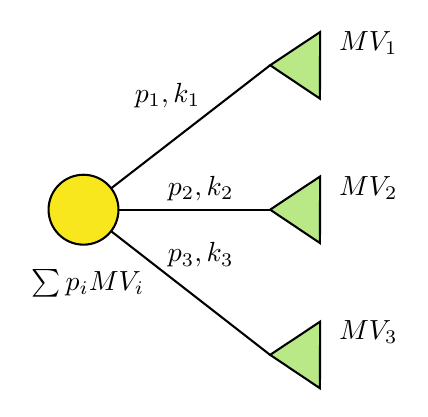
\begin{tikzpicture}[x=0.75pt,y=0.75pt,yscale=-0.8,xscale=0.8]
                		%uncomment if require: \path (0,300); %set diagram left start at 0, and has height of 300
                		
                		%Straight Lines [id:da9914598188026227] 
                		\draw    (125,128) -- (237.4,41) ;
                		%Straight Lines [id:da8494600211227674] 
                		\draw    (125,128) -- (237.4,215.45) ;
                		%Straight Lines [id:da3455826146339449] 
                		\draw    (125,128) -- (237.4,128) ;
                		%Shape: Circle [id:dp4694470217534936] 
                		\draw  [fill={rgb, 255:red, 248; green, 231; blue, 28 }  ,fill opacity=1 ] (103.95,128) .. controls (103.95,116.37) and (113.37,106.95) .. (125,106.95) .. controls (136.63,106.95) and (146.05,116.37) .. (146.05,128) .. controls (146.05,139.63) and (136.63,149.05) .. (125,149.05) .. controls (113.37,149.05) and (103.95,139.63) .. (103.95,128) -- cycle ;
                		%Shape: Triangle [id:dp6993619331790251] 
                		\draw  [fill={rgb, 255:red, 184; green, 233; blue, 134 }  ,fill opacity=1 ] (237.4,41) -- (267.48,21.01) -- (267.39,61.11) -- cycle ;
                		%Shape: Triangle [id:dp5948591148628843] 
                		\draw  [fill={rgb, 255:red, 184; green, 233; blue, 134 }  ,fill opacity=1 ] (237.4,127.97) -- (267.48,107.98) -- (267.39,148.08) -- cycle ;
                		%Shape: Triangle [id:dp600205010959115] 
                		\draw  [fill={rgb, 255:red, 184; green, 233; blue, 134 }  ,fill opacity=1 ] (237.4,215.42) -- (267.48,195.43) -- (267.39,235.53) -- cycle ;
                		
                		% Text Node
                		\draw (154,50) node [anchor=north west][inner sep=0.75pt]    {$p_{1}, k_1$};
                		% Text Node
                		\draw (174,106) node [anchor=north west][inner sep=0.75pt]    {$p_{2}, k_2$};
                		% Text Node
                		\draw (174,146) node [anchor=north west][inner sep=0.75pt]    {$p_{3}, k_3$};
                		% Text Node
                		\draw (277,19) node [anchor=north west][inner sep=0.75pt]    {$MV_{1}$};
                		% Text Node
                		\draw (277,106) node [anchor=north west][inner sep=0.75pt]    {$MV_{2}$};
                		% Text Node
                		\draw (277,193) node [anchor=north west][inner sep=0.75pt]    {$MV_{3}$};
                		% Text Node
                		\draw (92,162) node [anchor=north west][inner sep=0.75pt]    {$\sum p_{i} MV_{i}$};
                	\end{tikzpicture}
                	\label{ris:chance_node}
                	\caption{Графическое представление для вычисления EMV}
                \end{figure}
             
             \end{center}
        \end{column}
    \end{columns}


\end{frame}
% ---------------------------------------------------------------------------------------------
\begin{frame}{EMV - пример}

	Рассмотрим задачу строительства новой скважины на месторождении с заданными параметрами, тогда дебиты скважины могут оценены из выражения
	
	
	\begin{equation}
		Q = \frac{kh}{18.41 \mu B} \frac{\Delta P}{  \left( ln\dfrac{r_e}{r_w} + S\right) }
		\label{eq:eq_q}
	\end{equation}
	
	
	а доход от эксплуатации скважины в течении периода времени  $\Delta T$
	
	\begin{equation}
		MV = Q \cdot  \Delta T \cdot  Price_{oil} - Price_{well}
		\label{eq:eq_MV}
	\end{equation}

\end{frame}
% ---------------------------------------------------------------------------------------------
\begin{frame}{EMV - пример}

	Выражение \ref{eq:eq_MV} можно представить в виде
	
	\begin{equation}
		MV = \alpha k - \beta
		\label{eq:eq_MV_2}
	\end{equation}
	
	где 
	
	$$\alpha =  \Delta T \cdot  Price \cdot \frac{h}{18.41 \mu B} \frac{\Delta P}{  \left( ln\dfrac{r_e}{r_w} + S\right)}
	$$ 
	
	$$
	\beta = Price_{well}
	$$
	
	параметры, который мы предполагаем постоянными в рамках данной модели. 
\end{frame}


% ---------------------------------------------------------------------------------------------
\begin{frame}{EMV - пример}
	Тогда ожидаемую доходность с учётом неопределённости можно получить как математическое ожидание доходности с учётом заданного распределения. 
	
	\begin{equation}
		EMV = \sum_{i} MV \cdot P_i 
	\end{equation}
	
	Предположим, что  $\alpha = 1$, $\beta = 15$. 
	
	\begin{multline}
		EMV = \sum_{i} (\alpha k_i - \beta ) P_i = \\
		= (1 \cdot 10 - 15) \cdot 0.2 + (1 \cdot 20 - 15)\cdot 0.6 + (1 \cdot 30 - 15)\cdot 0.2 = 5
	\end{multline}

\end{frame}

\begin{frame}{Пример в виде дерева решений}
	
	\begin{center}
		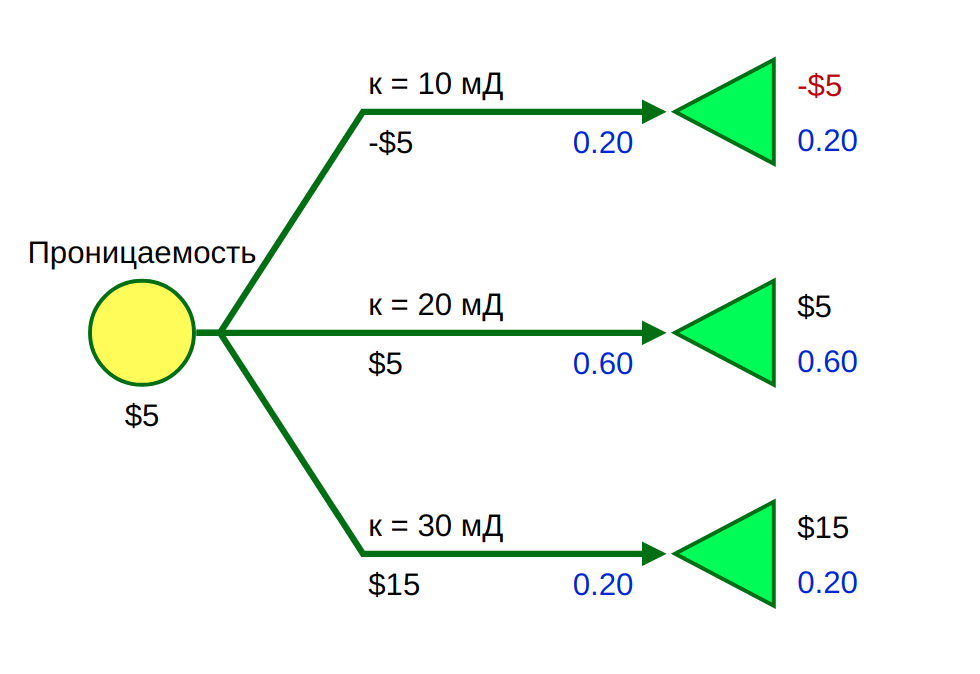
\includegraphics[width=0.6\textwidth]{pics/EMV_example_silversecision_1}
	\end{center}

	
	Пример построен с помощью сайта \url{http://silverdecisions.pl} 
	
\end{frame}



\begin{frame}{Как изменится EMV?}
	Как изменится EMV если провести гидродинамическое исследование?
	\begin{center}
		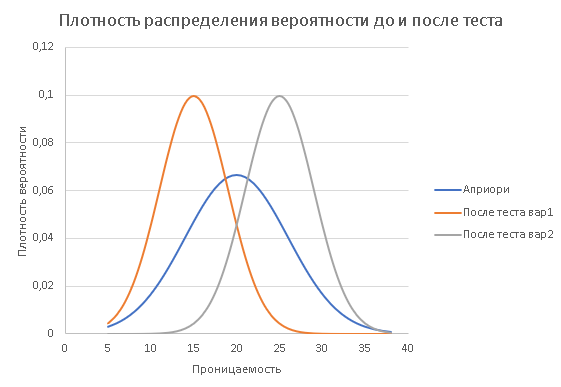
\includegraphics[width=0.6\textwidth]{pics_2/norm_distribution_ex1}
	\end{center}
	Предположим ГДИС может уменьшить разброс оценки проницаемости.
\end{frame}


%\begin{frame} 
	
%\end{frame}



\begin{frame}{Ожидаемые показатели после исследования}
	\begin{columns}
		\begin{column}{0.2\textwidth}
			\begin{center}
				Исход 1 ($p_1 = 0.5$)
				
				\begin{itemize}
					\item $k_1 = 10$ мД   $P_{1.1} = 0.2$; 
					\item $k_2 = 15$ мД   $P_{1.2} = 0.6$; 
					\item $k_3 = 20$ мД   $P_{1.3} = 0.2$. 
				\end{itemize}
			\end{center}
		\end{column}
		\begin{column}{0.2\textwidth}
			\begin{center}
				Исход 2 ($p_2 = 0.5$)
				
				\begin{itemize}
					\item $k_1 = 20$ мД   $P_{2.1} = 0.2$; 
					\item $k_2 = 25$ мД   $P_{2.2} = 0.6$; 
					\item $k_3 = 30$ мД   $P_{2.3} = 0.2$. 
				\end{itemize}
			\end{center}
		\end{column}
		\begin{column}{0.6\textwidth}
			\begin{center}
				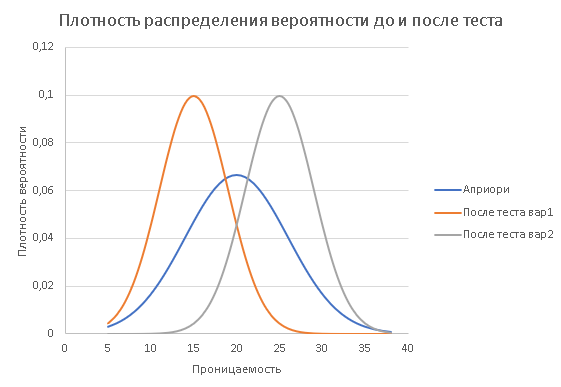
\includegraphics[width=1\textwidth]{pics_2/norm_distribution_ex1}
			\end{center}
		\end{column}
	\end{columns}
	
	Пусть $\beta = 18$
\end{frame}	

\begin{frame}{Пример в виде дерева решений}
	
	\begin{center}
		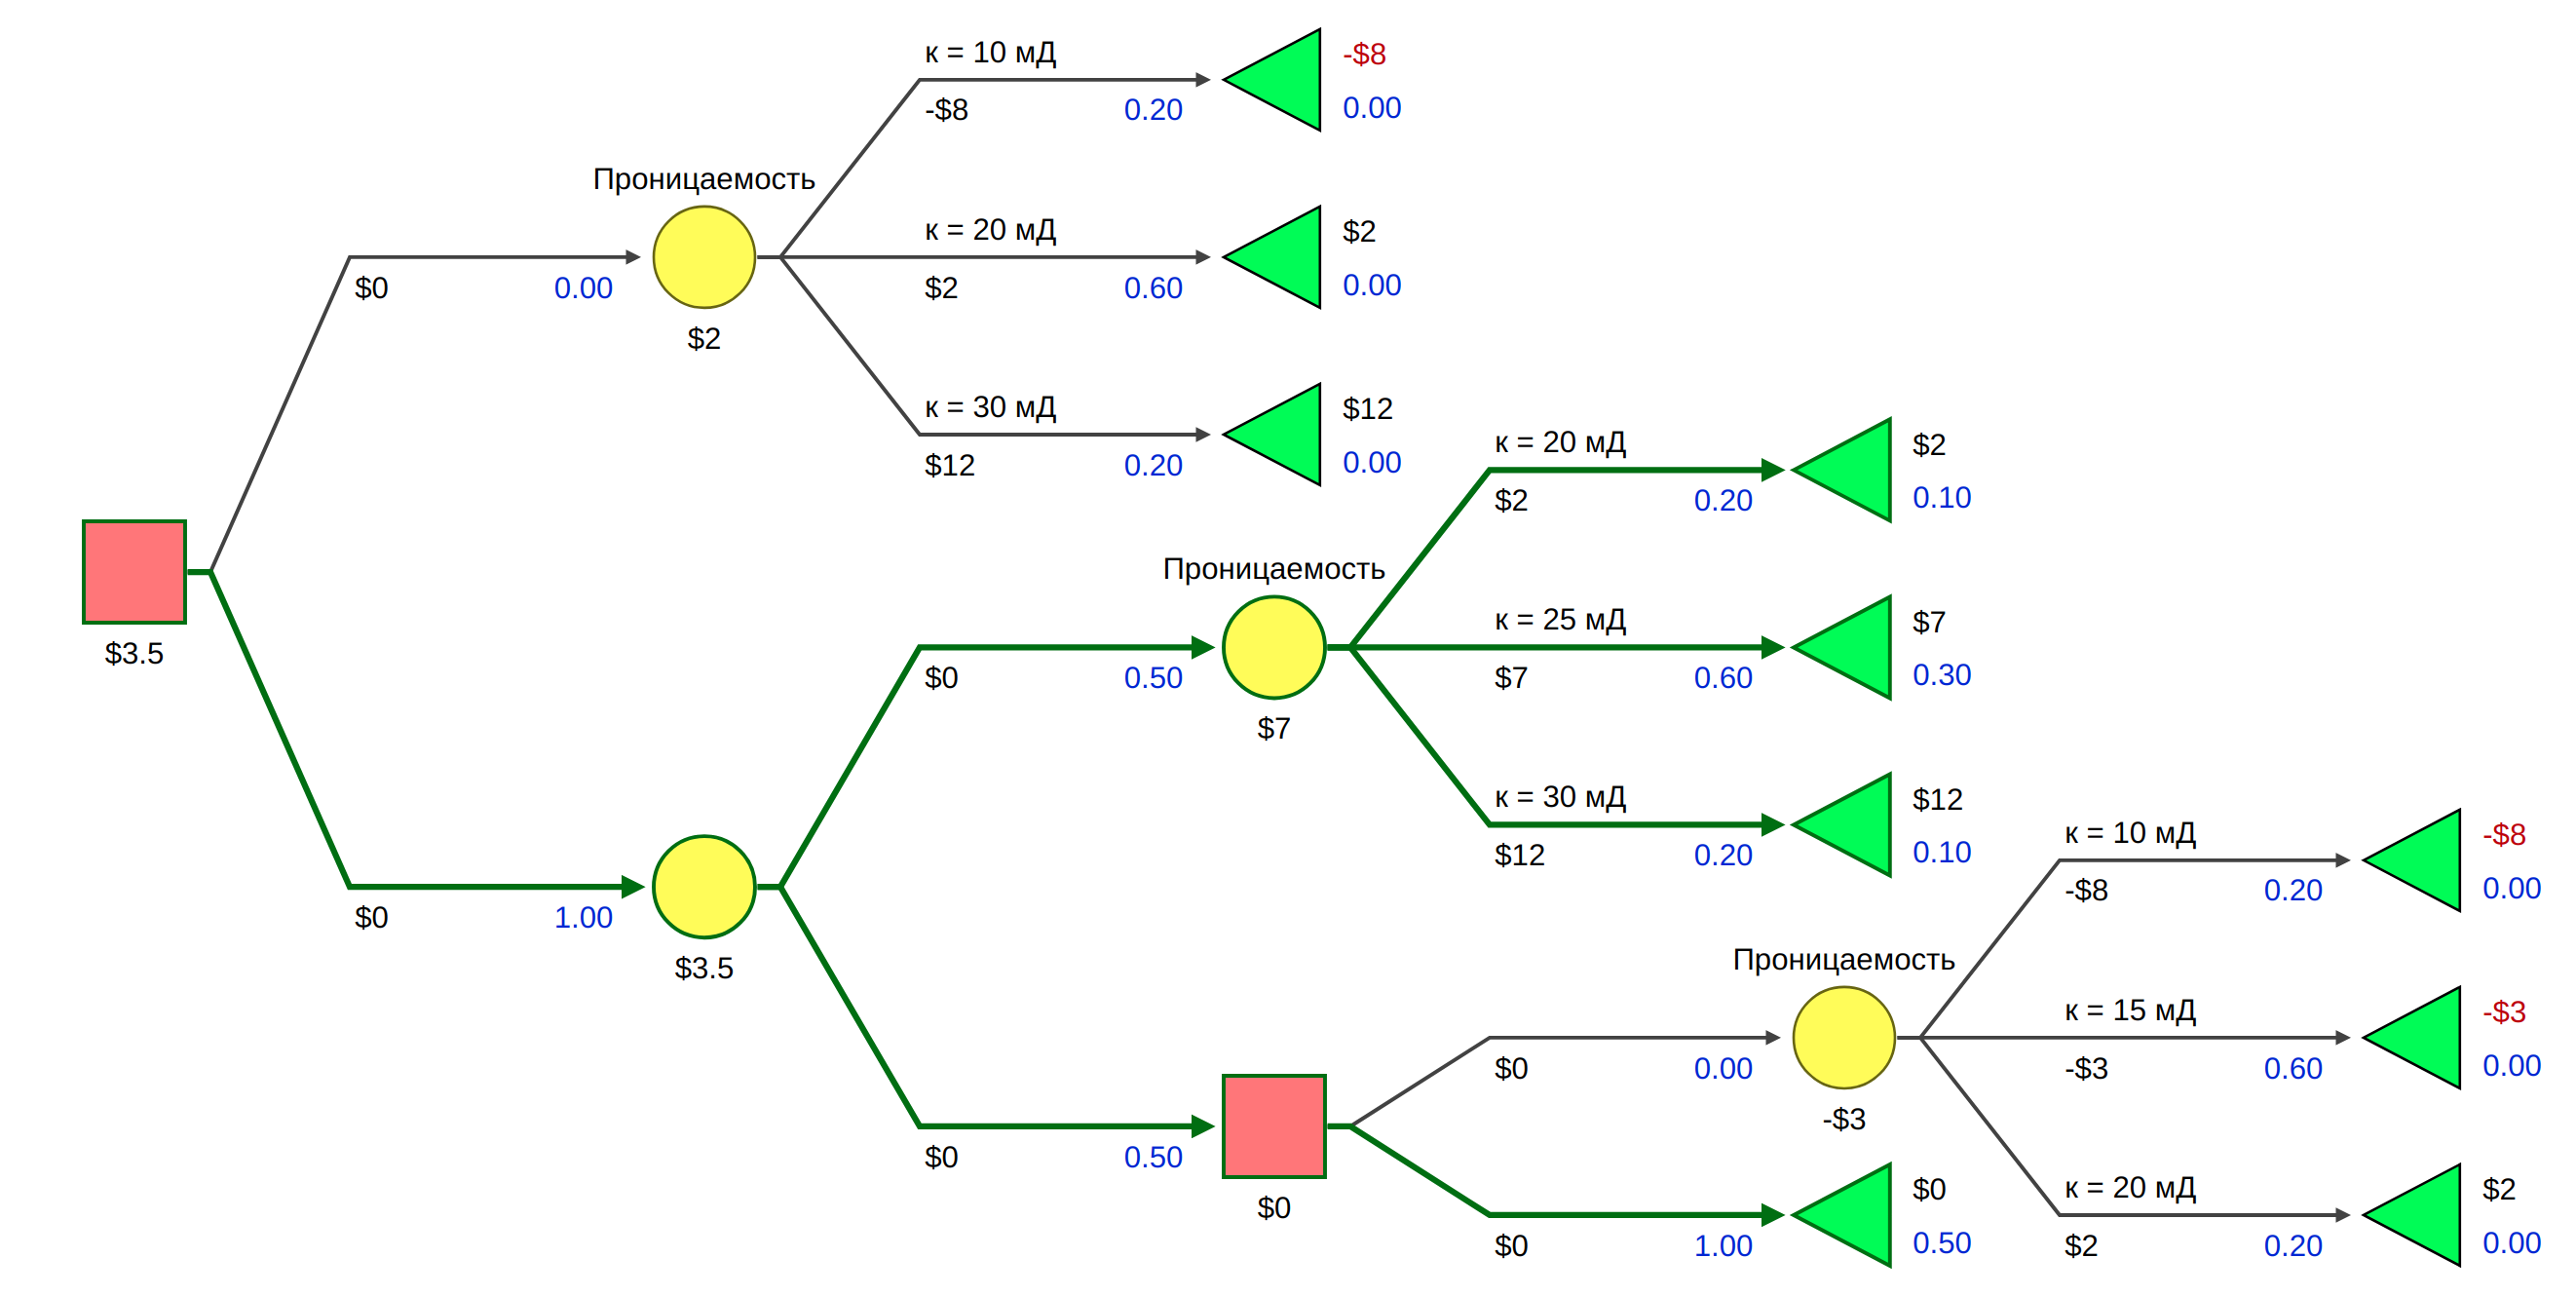
\includegraphics[width=0.9\textwidth]{pics/EMV_example_silversecision_2}
	\end{center}
	
	
	Чему равна ценность исследования VOI?  
	
\end{frame}

\begin{frame}{VOI - условия когда можно считать}
	- можно посчитать 
	
	- меняет решение
	
	- надо посмотреть в книге и дать ссылку на книгу также
\end{frame}